\documentclass[letterpaper, 10 pt, conference]{ieeeconf}  
\IEEEoverridecommandlockouts                             
\overrideIEEEmargins
\usepackage[utf8]{inputenc}
\usepackage[T1]{fontenc}
\usepackage{graphicx}
\usepackage{hyperref}
\usepackage{dirtree}

% The following packages can be found on http:\\www.ctan.org
%\usepackage{graphics} % for pdf, bitmapped graphics files
%\usepackage{epsfig} % for postscript graphics files
%\usepackage{mathptmx} % assumes new font selection scheme installed
%\usepackage{mathptmx} % assumes new font selection scheme installed
%\usepackage{amsmath} % assumes amsmath package installed
%\usepackage{amssymb}  % assumes amsmath package installed

\title{\LARGE \bf
Enterprise Backend as a Service(EBaaS)
}

\author{Aditya Doshatti$^{1}$ Darshil Kapadia$^{2}$ Devashish Nyati$^{3}$ and Maulin Bodiwala$^{4}$% <-this % stops a space
% \thanks{*This work was not supported by any organization}% <-this % stops a space
% \thanks{$^{1}$H. Kwakernaak is with Faculty of Electrical Engineering, Mathematics and Computer Science,
%         University of Twente, 7500 AE Enschede, The Netherlands
%         {\tt\small h.kwakernaak at papercept.net}}%
% \thanks{$^{2}$P. Misra is with the Department of Electrical Engineering, Wright State University,
%         Dayton, OH 45435, USA
%         {\tt\small p.misra at ieee.org}}%
}


\begin{document}



\maketitle
\thispagestyle{empty}
\pagestyle{empty}


%%%%%%%%%%%%%%%%%%%%%%%%%%%%%%%%%%%%%%%%%%%%%%%%%%%%%%%%%%%%%%%%%%%%%%%%%%%%%%%%
\begin{abstract}

In the world where we have computers and world wide web, web applications have become more and more popular. There has been a constant decrease in installed applications with people mostly relying on web applications to get their work done. With constant innovations in the field of computer, we see tons of startups everyday and what better option do they have than reaching to million people with a web application of their own. Talking about web applications we usually have 1) Frontend: what a user can see on their screen while accessing that web application and 2) Backend: what frontend communicates with to process the users’ requests. Since the invention of RESTful web services, developers have relied on APIs to which frontend sends request to in order to get an appropriate response. RESTful APIs have become more of a standard in developing the backend and more often than not, they are pretty basic with only queries changing to get data from the database. This paper provides a solution to automate the development of backend and thus doesn’t need any expert knowledge other than the knowledge of the underlying database and hence even a non-developer or a developer with no prior experience in developing backend can easily get access to the backend. The solution discussed here will ask user to provide database details and will create the database along with the downloadable code for backend which will be ready to use to interact with the frontend and the database.

Index Terms -- REpresentational State Transfer(REST), Backend, Frontend, Application Program Interface(API)

\end{abstract}


%%%%%%%%%%%%%%%%%%%%%%%%%%%%%%%%%%%%%%%%%%%%%%%%%%%%%%%%%%%%%%%%%%%%%%%%%%%%%%%%
\section{INTRODUCTION}
Web Application is nothing but a piece of software running on a remote computer which can then be accessed by anyone and at anytime over the internet. The idea of not having the code on our local computer and still be able to access it has played a major role in people accepting the trend of web applications. But this development of web applications would not have been this popular if the concept of RESTful(REpresentational State Transfer) system had not come into the picture. REST system was introduced as a protocol for exchanging data over the internet and by doing so revolutionized the development of web services. As discussed above, web application is majorly comprised of frontend and backend. Frontend deals with how the data should be shown to the user and backend deals with what data needs to be shown. In the past when REST system wasn't introduced, people were controlling the data on the frontend side and in turn making the whole process heavy. Since the introduction of REST and RESTful APIs, developers have started to design the functionalities as APIs which will then be consumed on the frontend. This separate piece of RESTful code is major part of the backend. In today's world, one can see no projects that doesn't use the RESTful system for the creation of professional web services. Major companies like Yahoo, Facebook, Google, and many more do business on their RESTful APIs.

So the next question can be, what is RESTful API and what does it do? If thought at a very basic level, API is going to control what data will the frontend show and what operations need to be done on that data. The data can be static but most usually API communicates with the database to manipulate on the data. To understand it in the real world, let's take an example of Airbnb. The most basic thing a user do on Airbnb is searching for a property and when a user request the application to show him/her properties in a particular region and in a date range, then that information is sent to the API which manipulates the database to find all the properties which satisfy the user's requirements. This API uses the GET method of Hyper Text Transfer Protocol(HTTP) since it is just getting the data from the database. But one can think, how was the database populated in the first place. For that, API which uses POST method of HTTP is used by the frontend to post a new property into the database. Not just that, using PUT method APIs can edit the already stored data in the database i.e for changing the price of already posted property. To remove a property, DELETE method is used by the API to remove that record from the database. This was an example of Airbnb but the same things can be visualized in other applications too like Grubhub, Facebook, and many more. So if thought at a lower level, it all comes down to interacting with the database using queries and the normal CRUD(Create, Read, Update and Delete) operations are a must when it comes to developing any web application.

In the world of startups, the need for fast development of applications is rising. Companies constantly urge developers to create applications and other business software more quickly without sacrificing quality. In such situation, having a solution which provides RESTful APIs on the go based on the database details can be seen as a blessing. To address this situation, this paper provides a solution by offering enterprise backend as a service. The solution discussed in this paper communicates with the user to get their requirements in terms of database and takes care of the tasks like creating the database, hosting the database and creating a CRUD based RESTful APIs and providing the code for the same. Along with that, the solution also provides machine learning based RESTful APIs for the enterprise businesses to get insight into their data. Small organizations or start ups face problems in creating back-end API’s and hosting the server on cloud platforms. Automated generation of back-end API’s can save a lot of time. It can benefit not only IT experts but non IT people also. It can help back-end developers, front-end developers, data scientists and non technical people as follows:
\begin{itemize}
\item``Back-end Developers'': It can help back-end developers to create databases, quickly create API’s by auto generation, modify the API’s if needed and quickly host the server on some cloud platform.
“Front-end Developers: It can save a lot of time for front-end developers who needs backend API’s and databases hosted on a cloud platform.
\item``Data Scientists'': It can help data scientists and machine learning engineers as they can quickly save data into databases using API’s, add on the API’s for their purpose.“
\item``Non Technical People'': It can be a life saver for non technical people as they can create databases using this, create and host a server with RESTful API’s, connect with a machine learning service. Later they can even use the code to extend the functionalities.

\end{itemize}


\section{RELATED WORK}
A key factor driving business growth is the need to minimize nuances in the development of applications. Backend as a service reduces the subtleties of mobile and web applications development and design. It eliminates the need for application developers to create their own server interaction process backend system. Backend-as-a-service vendors offer solutions that do not require complex coding for server hosting, which reduces application development time and improves frontend tasks such as application design and user interface (UI) design.[1] In the paper “Availability Evaluation and Sensitivity Analysis of a Mobile Backend‐as‐a‐service Platform”, Costa, Igor, Jean Araujo, Jamilson Dantas, Eliomar Campos, Francisco Airton Silva, and Paulo Maciel have explained how backend as a service enables engineers to connect their application backend to cloud servers. They also explain, how backend as a service can be used to integrate with other apps.[2]
After gaining understanding of backend as a service we dig deep to understand different type of structures in Databases as Databases are the integral and most important part of any system if you are focusing on Database. In the research paper. Having a look towards a REST-based Universal API for Database-as-Service Systems, "Till Haselmann explained that the objectives of the API should be to provide maximum flexibility and exchange-ability, for which the relational databases operate as the greatest source and we should, therefore, use the SQL database.To support this thought we found that in “A relational database environment for numerical simulation back-end storage” Jacek Nazdrowicz also supports the thought of using SQL databases for back-end[3][4].
A few efforts have been made to understand relation between Model Driven Engineering and Web Engineering which normally called Model Driven Web Engineering which proposes the utilization of the models and model changes for the specification and semiautomatic age of Web applications [6][8][9]. Most of the projects have essentially utilized information models, route models and presentations models to automate the process of the Rest API Creation. [11] [17] [18] most of them are providing features of creating web services but generating the REST-ful APIs is very less and even if they are providing APIS the approach require us to model the APIs in specific DSL from which it generates the APIs. Going forward one more step EMF-REST [19][20] approach generates REST-ful web APIs from EMF models. This implementation has filled the gap between Modeling methodology and web technologies. The Eclipse Modeling Framework also has one limitation that it does not provides the Code which has it’s own limitation of maintenance.There are also several approaches explored about generating REST API from a legacy application which follows a common process of reverse engineering of L-System to REST-ful APIs[8]. It is also having the same limitation they are not providing any code which comes which one more limitation of maintenance and future changes.
This project generates the REST-ful APIs from the MODELs which is also one of the adaptation of Model Driven approach, with an added advantage of the access to the automatecally generated REST APIs.Which helps the stack holders to deal with the real code and make the changes based on their requirements.
Code Generation as a servise uses Epsilon [5] to perform model-to-text transformations,the generated output can be utilized for any language and the service is being implemented with an API, so any client program can do the maximum use of it.[21] which is one more improvement this project is doing. Our Project is removing the requirement of Epsilon and also providing a complete code in proper folder and file structure which can be utilized or maintained by the client. 


\section{PROJECT OVERVIEW}
\subsection{Problem Statement}
As explained in the above section, backend is a middleware that handles the functionality of an enterprise application via API or SDK.  Backend as a Service allows users to maintain only the frontend with everything behind the scenes aspects related to the backend being managed by the service model. 

Our problem statement is to build an application that will interact with the user to create a backend code that should create the required product with bare minimum requirements starting from the creation of the database to the creation of the APIs to communicate with the database. The user should be able to build applications in a few minutes with just a few clicks. The user should be able to achieve 3 main goals:
\begin{itemize}
  \item Build Application:
  The user should build the backend applications with just a few clicks and be able to host them on different cloud services.
  \item Generate Code:
  The user should be able to generate the backend code without having any prior knowledge of coding.
  \item Build Databases:
  The user should be able to migrate their existing databases or create new databases easily using our application.
\end{itemize}

\subsection{Project Architecture}
The project architecture can be divided into 3 parts. The first part is the user interaction part as shown in Fig. 1. Here we would have a website wherein user would input data in forms. The user would be able to give their specifications and details using these forms. After collecting the input in the second part we have the EBaaS server, where our code would process the inputs and generate the database with the schema on the user provided database server and generate the code for APIs for the same and publish a docker image with the code for the code. 

\begin{figure}[h]
   \centering
   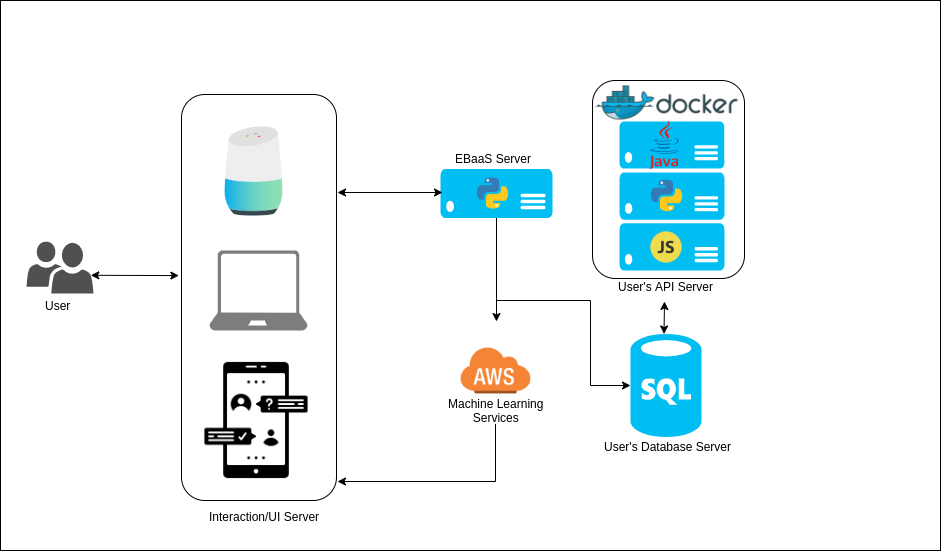
\includegraphics[scale=0.23]{./ArchDiagram.png}
   \caption{Architecture Diagram}
   \label{fig:my_label}
\end{figure}

We plan to use the machine learning services provided by AWS to suggest the data points which user should consider adding to their schema to make it more good. The output would be a published docker image which the user can download and spawn a container out of it on its API server. The container will also have the code so the user can get into the container and customize the code if he/she wishes to do so.


\section{METHODOLOGY}
This section of the paper describes the process that goes behind bringing the idea of Enterprise Backend as a Service into existence. The project aims for allowing user to control the information from nothing but just the mere knowledge of the user of what information he/she wants to manage. Putting it in a technical context, the project is trying to provide the user with a backend that gives control to the models which are nothing but a representation of the information the user wanted to manage. Breaking it into various processes, two major processes stand out 1) Generating the models from the information the user provides and 2) Generating the actual backend to control those models. 

For simplicity, lets discuss a use-case where the user would feel the need to use this project and how the project works for that particular use-case. Consider a situation where a user is tasked with building a prototype of a employee management system within an organization in a short span of time. Now, the user would be needing models which can than be translated into a database system and obviously an application which can handle basic operations like creating, retrieving, updating and deleting of resources of a particular model. This will be the first and the most basic requirement that the user would have to kick start the more complex operations on the models. In fact for that matter, any model driven system would need an application which can handle the basic CRUD(Create, Retrieve, Update, Delete) operations as a starting point. Now, in this particular situation the user could either opt to design the application that handles CRUD operations which could take up a substantial amount of time for something very basic but important. Or the user could opt for a solution which could provide this basic application on hand with nothing but the information about the model. This is where this project comes into the picture to make life easier for that user and saving the user’s days of designing.

Before digging deep into the major processes discussed above. lets discuss about the actual application that the user would interact with for obtaining results. The application runs on a load balanced EC2 instances on Amazon Cloud Service which is hosting the application’s front-end developed in JavaScript and ReactJS framework and back-end which is developed using Python and Flask Framework. The user would be presented with a login screen on a startup and hence allows the application to manage each and every user’s projects separately and securely from one another. This calls for the need of the database which is a SQL database hosted on Amazon Web Service’s RDS service. Coming to the security, the actual application never really stores the database records anywhere within the whole system and only helps users to create a database in the first place. After the creation, the user has full access to the database without the actual application having any access to that. So, now its time to dig deep into the major processes.
\subsection{Generating Models}
As discussed above, the first thing the user would want in this use case would be the models which can be mapped to and from the database system. The actual application never gets too harsh with the user which can be proved by the way the application asks the information from the user. Let’s say that the user in this case has no idea of what different kinds of information the organization wants to manage except for the employee’s name and salary. To handle such cases, the application presents user with the User Interface which asks information progressively.

\begin{figure}[h]
   \centering
   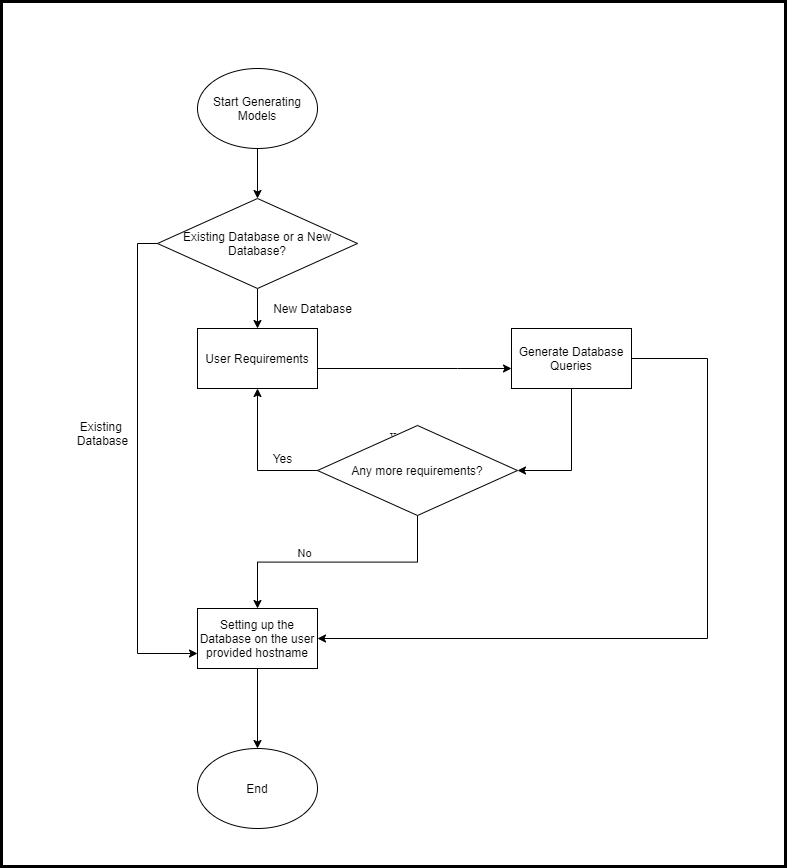
\includegraphics[scale=0.25]{./Models2.png}
   \caption{Generation of Models - Workflow}
   \label{fig:my_label}
\end{figure}

The very basic thing the user would need over here is the server where the database can be hosted. This again brings forward the point that once the database and the back-end is created, none other than the user will have access to that database’s records. So, the application will put forward 4 options to the user allowing him/her to connect to the database viz. 1) Create a new database 2) Connect to an existing database 3) Connect to a database using Excel and 4) Connect to a database using SQL file. In this case, lets assume that there is no existing database that the user has and selects the first option of creating a new database. As shown in the Fig. x, the application would ask user to enter details like host-name, username, password, database name and connection name. Connection name is required to extinguish multiple connections to various databases the user connect to. This would result into a database creation on the server hosted by host-name. Didn't that feel like a magic? Behind the scenes, this operation of the user would result in a request hitting the application’s back-end which does nothing but executes the required commands to connect to the host and creating a database. User has decided to create a new database called “test” locally denoted by localhost as the database address in Fig. 3. On submitting the request the application would create a database named “test” with privileges given to the user “root” with no tables which can been seen in Fig. 4.

\begin{figure}[h]
   \centering
   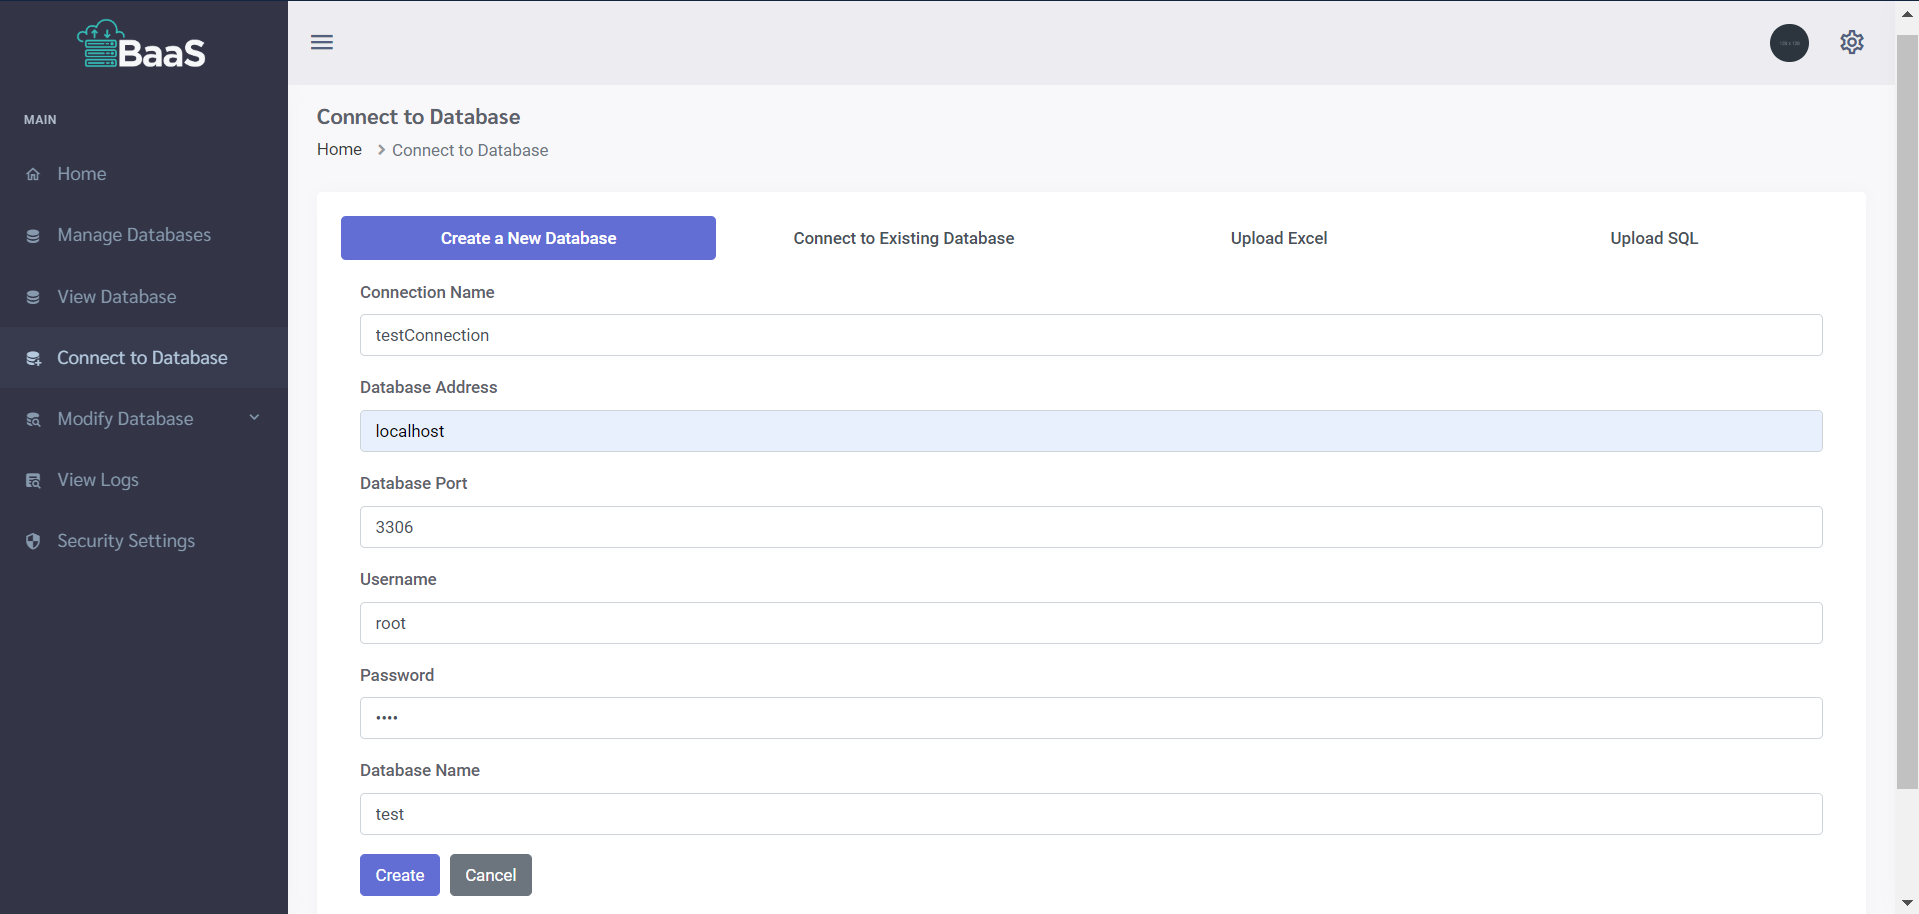
\includegraphics[scale=0.17]{./fig1.png}
   \caption{Create database form}
   \label{fig:my_label}
\end{figure}

\begin{figure}[h]
   \centering
   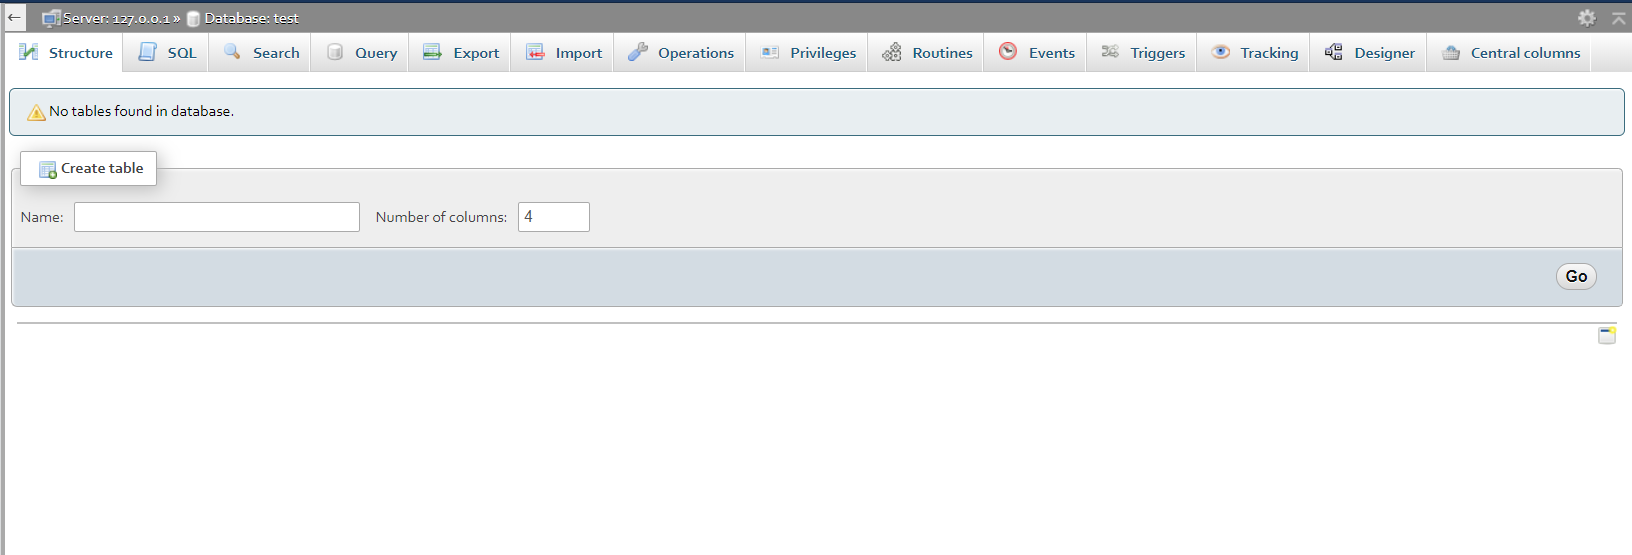
\includegraphics[scale=0.19]{./fig2.png}
   \caption{Corresponding database with no tables}
   \label{fig:my_label}
\end{figure}



Now, since the user in this case has created a new database there won’t be any tables present in that database. Hence, the next thing the User Interface presents to the user is a chance to create tables. As discussed earlier, the user only knows about managing employee’s name and salary and hence will suffice with creating only one table and on successful creation, the user will progress to add columns like name and salary.

\begin{figure}[h]
   \centering
   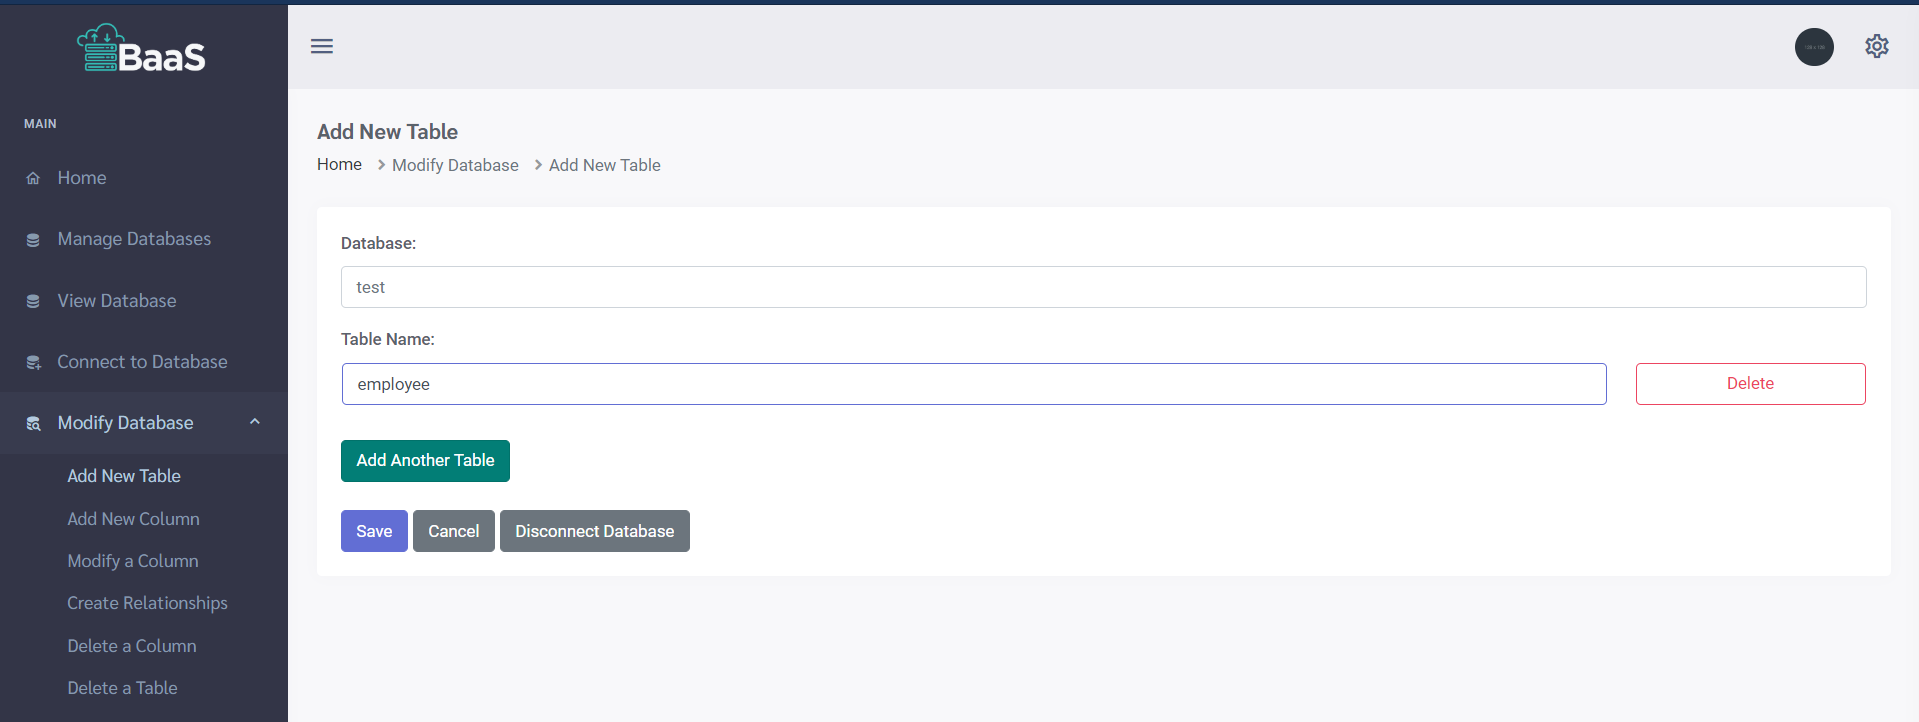
\includegraphics[scale=0.17]{./fig3.png}
   \caption{User Interface to add tables in a database}
   \label{fig:my_label}
\end{figure}

\begin{figure}[h]
   \centering
   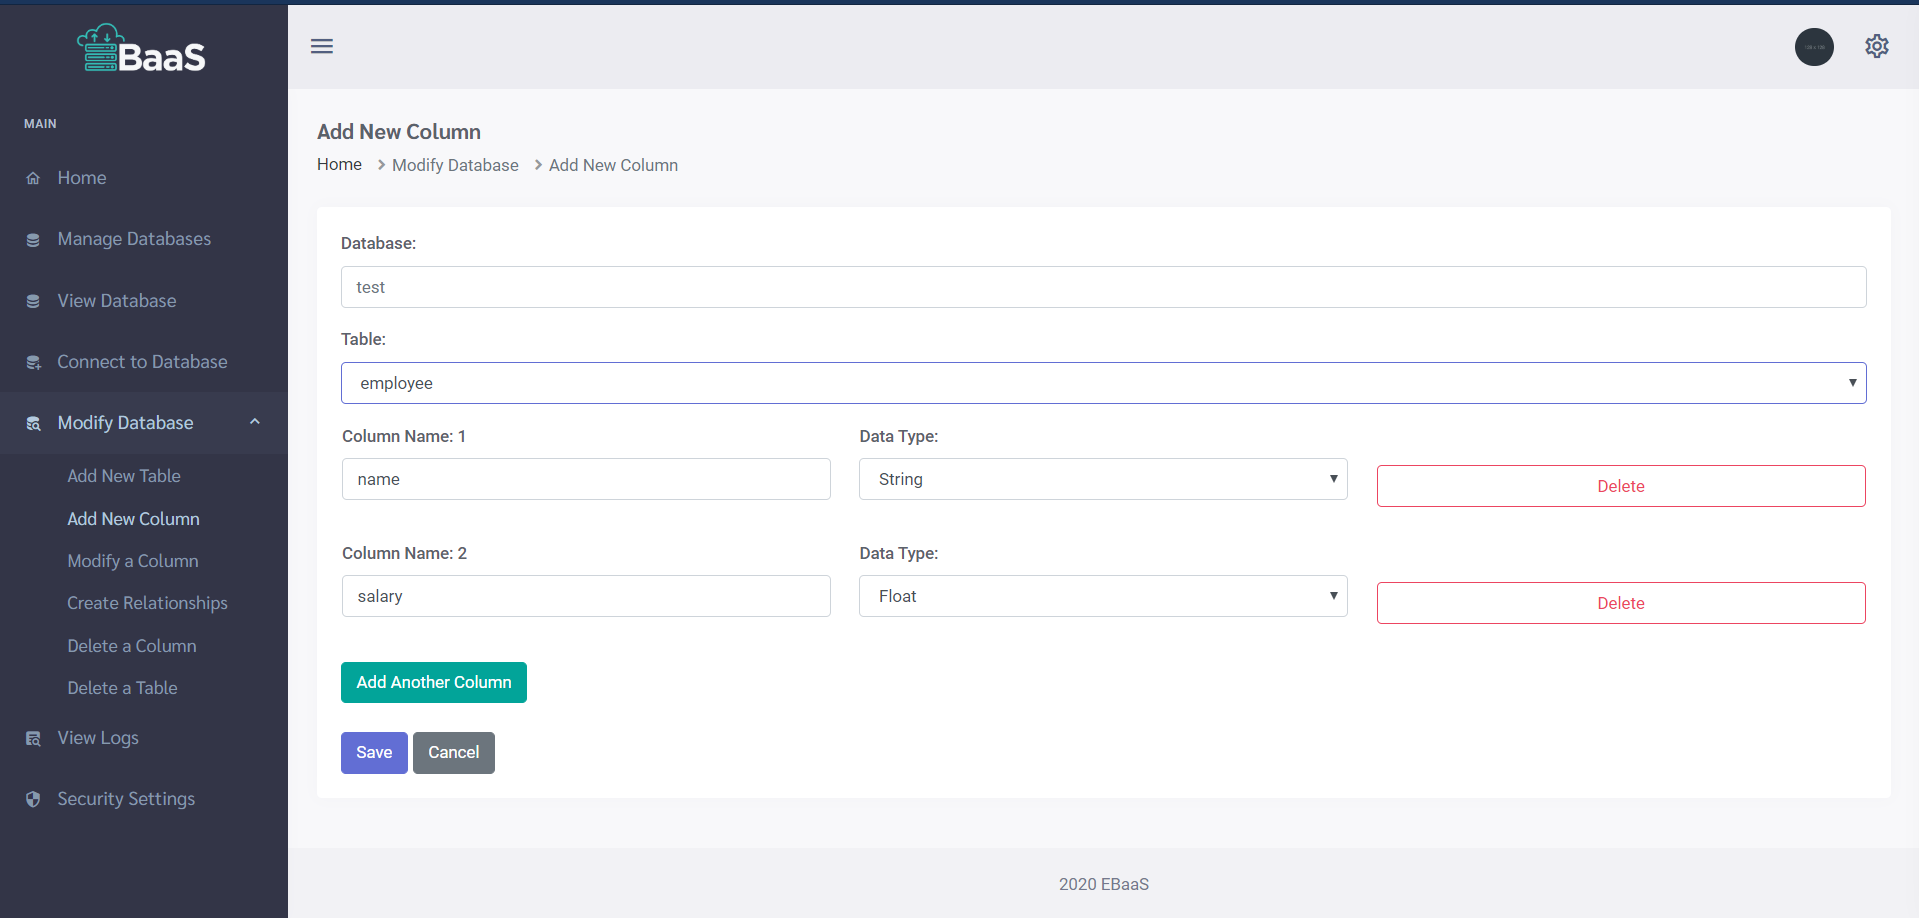
\includegraphics[scale=0.17]{./fig4.png}
   \caption{User Interface to add columns in a particular table}
   \label{fig:my_label}
\end{figure}

These operations would be presented to the user as shown in Fig. 5 and Fig. 6. Fig. 5 allows user to add tables and Fig. 6 allows user to add columns to the tables which the user selects from the drop-down of already available tables in the database. The corresponding change could be validated in Fig. 7.

\begin{figure}[h]
   \centering
   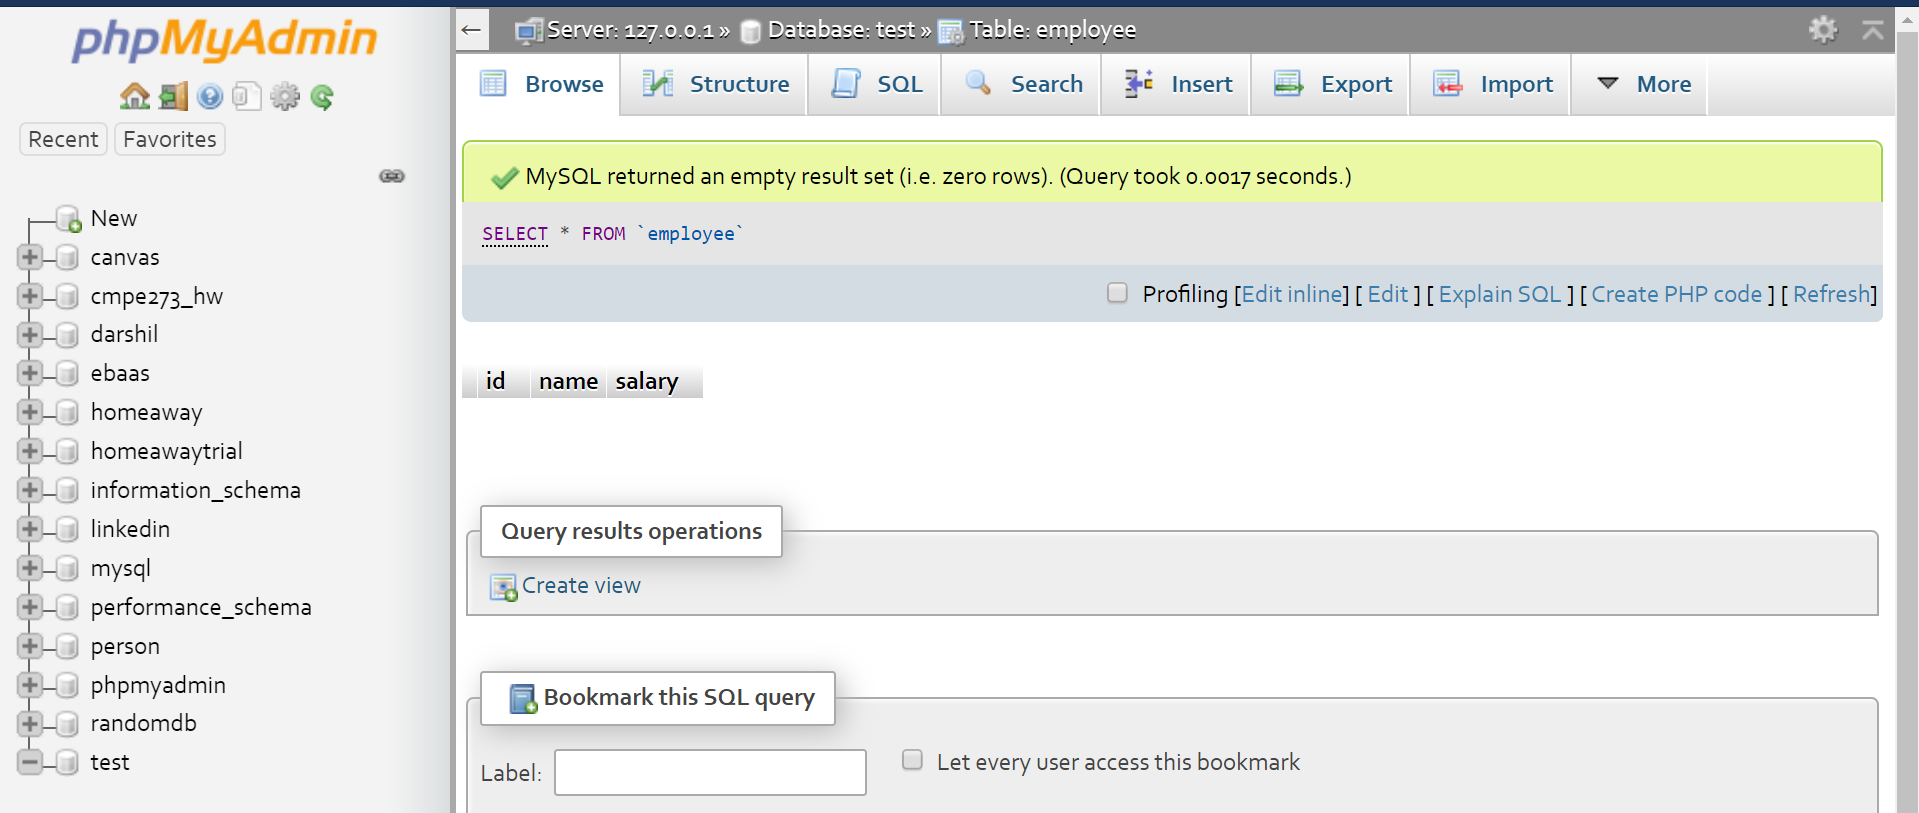
\includegraphics[scale=0.17]{./fig5.png}
   \caption{Corresponding change in database}
   \label{fig:my_label}
\end{figure}

By doing this, the user has provided the minimal requirements that it needs to launch an operation of creating a back-end. But what if the user is now informed that the organization wants to manage employee’s addresses too? In that case, the User Interface which has been designed for entering information progressively, allows user to add a new table in to the database and along with that establishing a relationship between those two tables. This again, behind the scenes would result in operations that executes SQL queries to reflect the user changes on the actual database.

This way the application generates the database model step by step. There is no ground breaking technique which the application is using here to generate these models but instead is focusing on operating and manipulating database models through simple SQL queries known to the whole world in a systematic and a more structural way. For example, the user’s request to add a new column to the table with specific data type would do nothing but trigger an “ALTER TABLE” query behind the scenes. The progressive way of asking the information from the user will make sure that the table “ALTER TABLE” is trying to alter already exists as the user would have been asked to create a table first before adding columns.

This database model will help in generating object oriented models which our back-end will be using to manipulate data within the database. Hence, the next step would be to map models out of these already created tables and generating the code to manipulate database through those models. That is where our next process of “Generating Code” comes into the picture.
\subsection{Generating Code}
Generating code is something that has brought that extra edge to this propose project. To be even more specific, this project aims to generate a back-end code with basic CRUD operations on the models. The first decision that had to be made over here is deciding over the service’s architectural style. With many architectural styles out there like SOAP, REST, RPC, GraphQL etc. the style which has dominated the market in the past decade has been the RESTful architectural style. The support of REST style is ever increasing and competence of using REST is something which every programmer is demanded for. 
\begin{figure}[h]
   \centering
   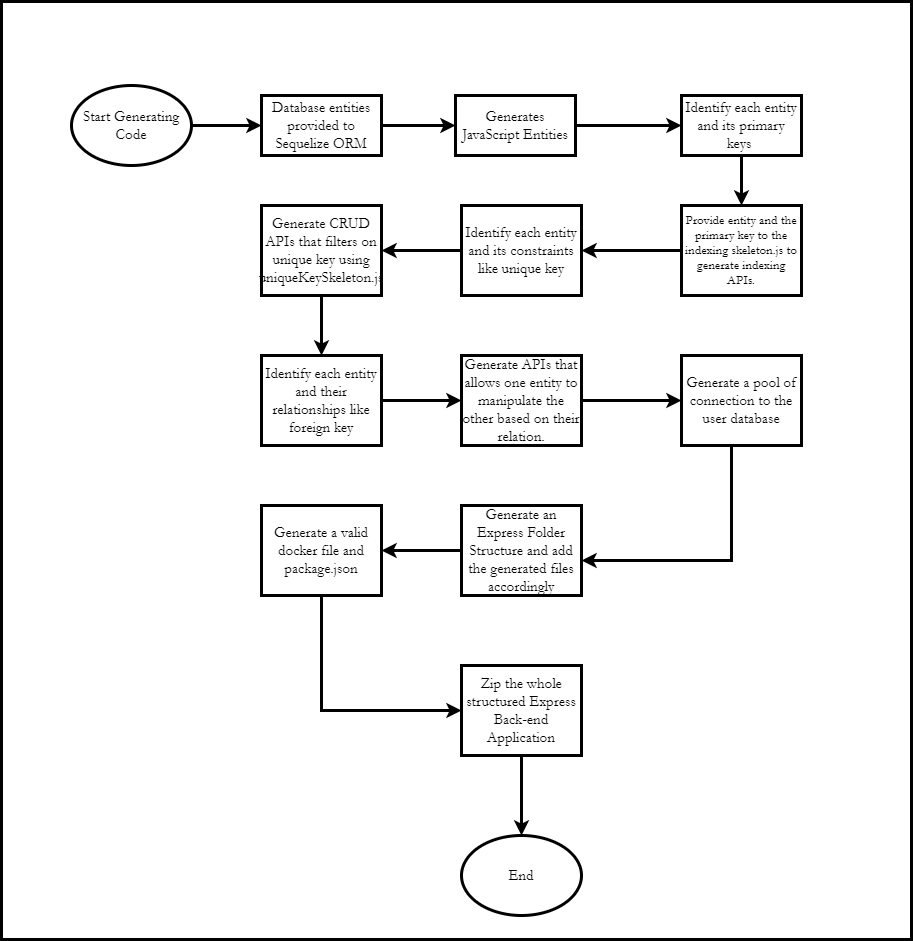
\includegraphics[scale=0.25]{./Code2.png}
   \caption{Generation of Code - Workflow}
   \label{fig:my_label}
\end{figure}
Not just that, majority of the web services in the past decade has been designed using RESTful architectural style. This was the major reason that drove the idea of generating a RESTful API as a back-end that will further manipulate with the database/models as it allows the project to target the maximum crowd out there. Once that decision was made, the next decision was to decide upon the programming language that the code will adhere to which in this case was decided as JavaScript.

Coming to the process of generating code, it is further divided into small processes like deciding a generated code’s file structure, mapping database system to JavaScript models, database connection, type of URIs etc. Lets discuss these processes one by one.
\subsubsection{File Structure}
Once the technology was decided as JavaScript, NodeJS was the clear option to go with as we were creating a server which the client could use to interact with the database. According to [14], the project decided to organize and present the files around features and not roles. Apart from that, a configuration file that would take care of all the configuration written in JSON and imported wherever necessary. This certifies the uniformity across the back-end code as any change in the configuration could be easily be made by changing only one file in the whole application. Lastly, the logic of each model is separated in the “routes” folder with "index.js" working as the router that routes to the correct file.

This file structure ensures the best practices are followed and brings modularity in terms of structure.

\subsubsection{Mapping Models}
Once the user submits the information through the application and wishes to launch an operation of generating the code, the mapping of database to JavaScript models becomes important. Models work as abstraction between the object oriented programming and the database which is generally called Object Relational Mapping(ORM).


\begin{figure}[h]
   \centering
   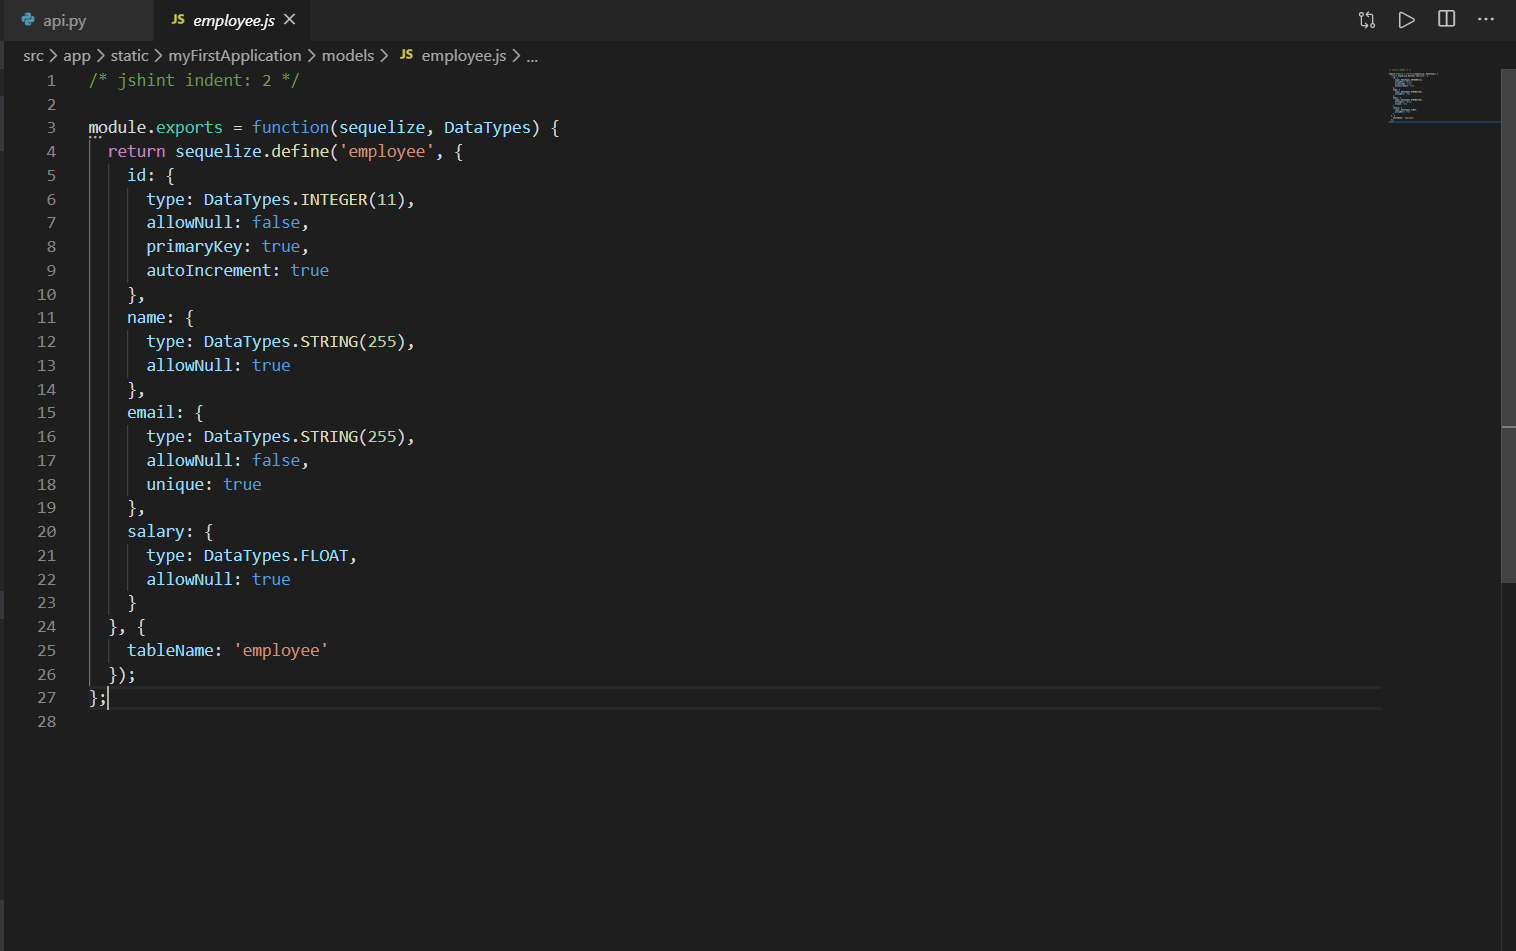
\includegraphics[scale=0.21]{./fig6.png}
   \caption{Employee model mapped from database}
   \label{fig:my_label}
\end{figure}

\begin{figure}[h]
   \centering
   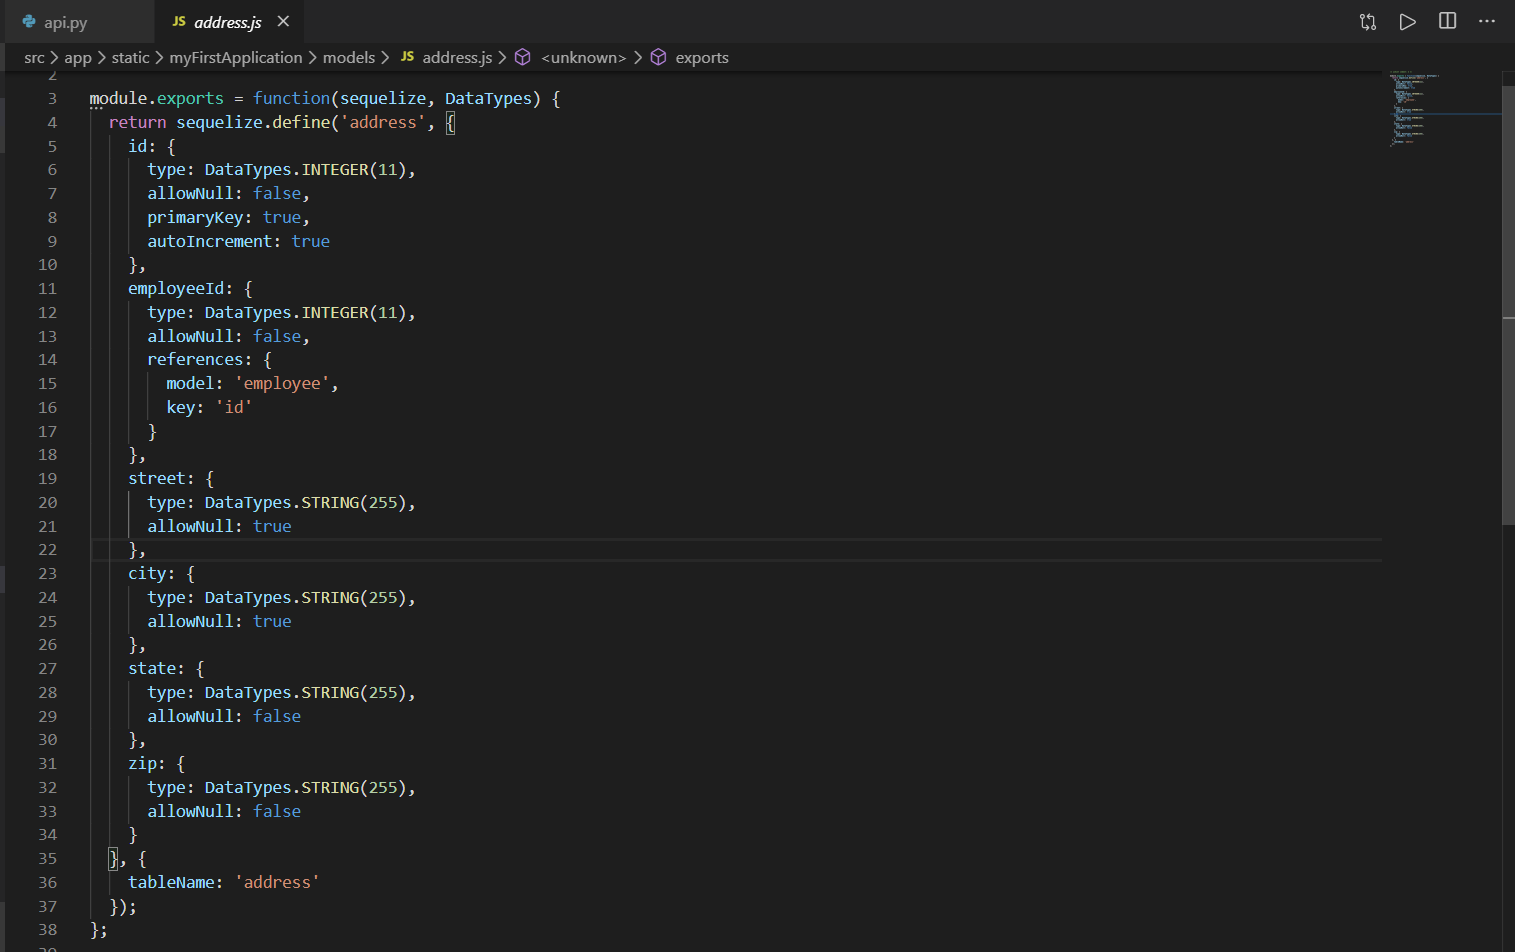
\includegraphics[scale=0.21]{./fig7.png}
   \caption{Address model mapped from database}
   \label{fig:my_label}
\end{figure}

This project uses Sequelize as the ORM and exploits the sequelize’s feature of auto generating the models through specified database using “sequelize-auto” command. Sequelize takes care of converting the database tables into the appropriate JavaScript object models. The table “employee” and "address" in the database has been converted to the JavaScript models as shown in Fig. 9 and Fig. 10.


\subsubsection{Database Connection}
Coming to the connection to the database, the project manages a pool of connection which eliminates problems related to connections like open connections. The configuration of the database like host-name, username, password and database name is stored in the configuration file for a single point of manipulation.

\subsubsection{URIs}
Selecting the URIs that the project would provide was the most critical part. The project only kept focus on providing CRUD operations in the generated code. But even then, updation, deletion and retrieval of the resources needs a parameter which acts as a filter on which the operation is going to get performed. For example, if there is an employee with ID as ‘1’ and if the user wants to change that employee’s name then the URI would be /employee/<id> where <id> will be replaced by 1 and the change would be made on only that particular employee. Hence, it works as a filter. But ID is said to be an identifier and more often than not this identifier is managed directly by the database. Hence it cannot be assumed that the user would always know the employee’s ID. 

Hence, giving only the identifier as the filter option would have made most CRUD URIs useless for the users and also it would have been a chaos if the project provided each attribute of the model for filtering purpose. Analyzing the situation, a middle ground had to be established. Looking at the employee model, it shows that “email” attribute is unique across all employees which could be exploited by the user for filtering through the employees. This very idea is put into effect in this project where the filter options includes identifiers like IDs and unique fields like email, name, etc.

Apart from that, URIs to honor the relationship between models are also provided. For example, one employee model record can hold many records of address model. So the user should be allowed to manipulate the child table(address) through parent table(employee). The example of one such URI is presented in Fig. 11.


\begin{figure}[h]
   \centering
   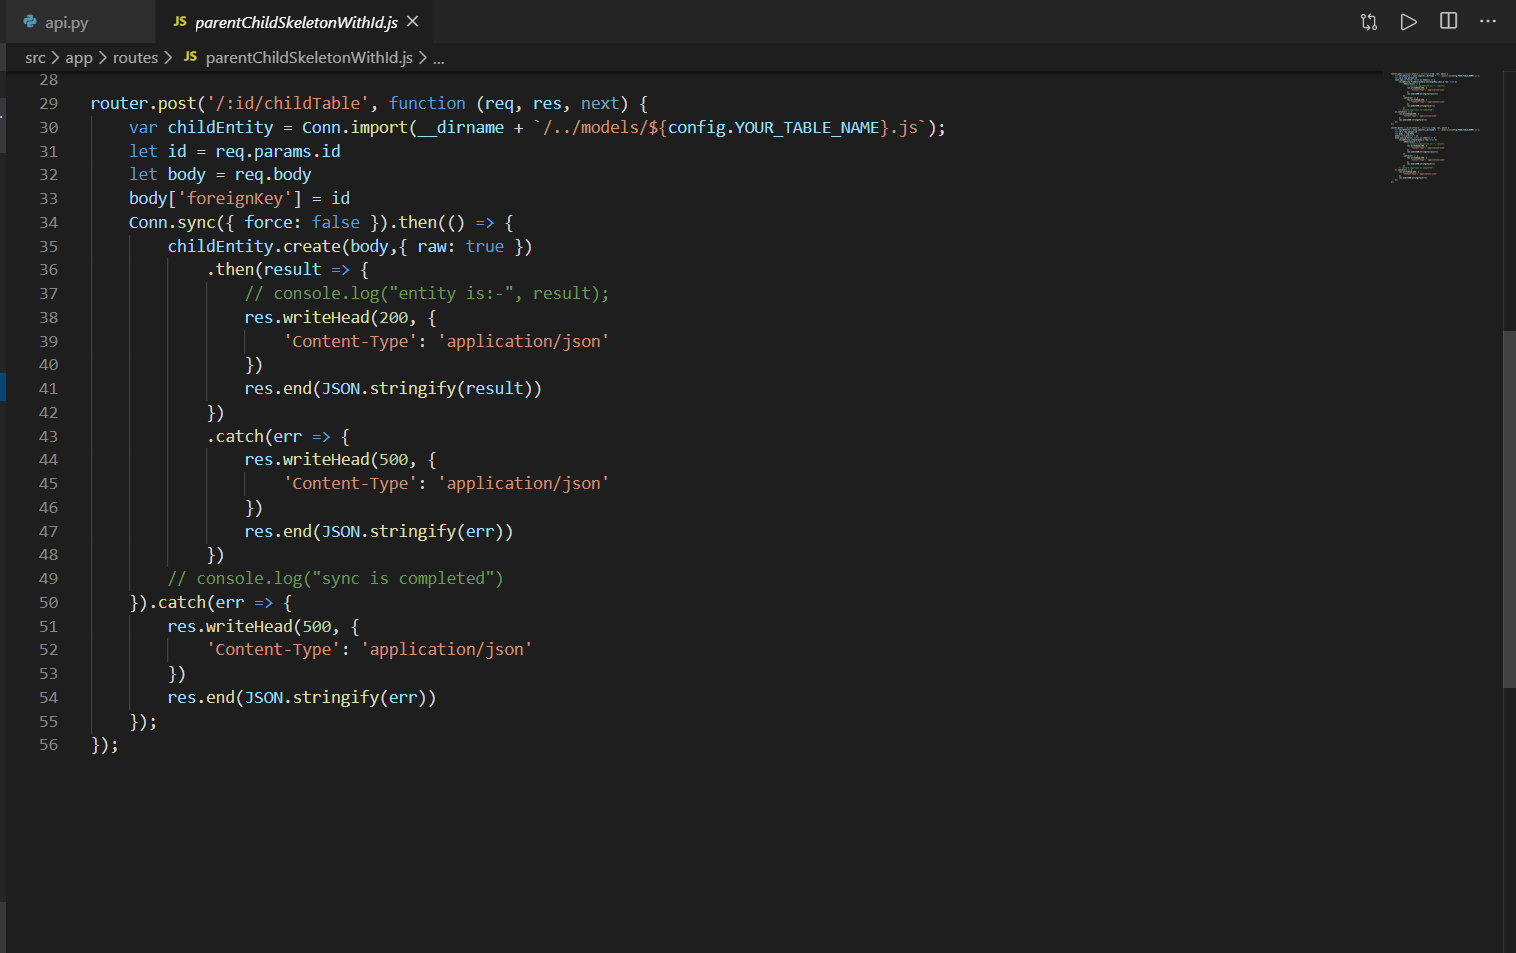
\includegraphics[scale=0.215]{./fig8.png}
   \caption{Skeleton for designing URI to connect child and parent table}
   \label{fig:my_label}
\end{figure}

Once the types of URIs were decided, the project digs deep into the database schema to find information about the structure like number of tables, columns in tables, relationship between tables etc. This information is then provided to the templates one by one to create the actual code from the template. An example of template and its corresponding actual code in shown in Fig. 11 and Fig. 12 respectively.


\begin{figure}[h]
   \centering
   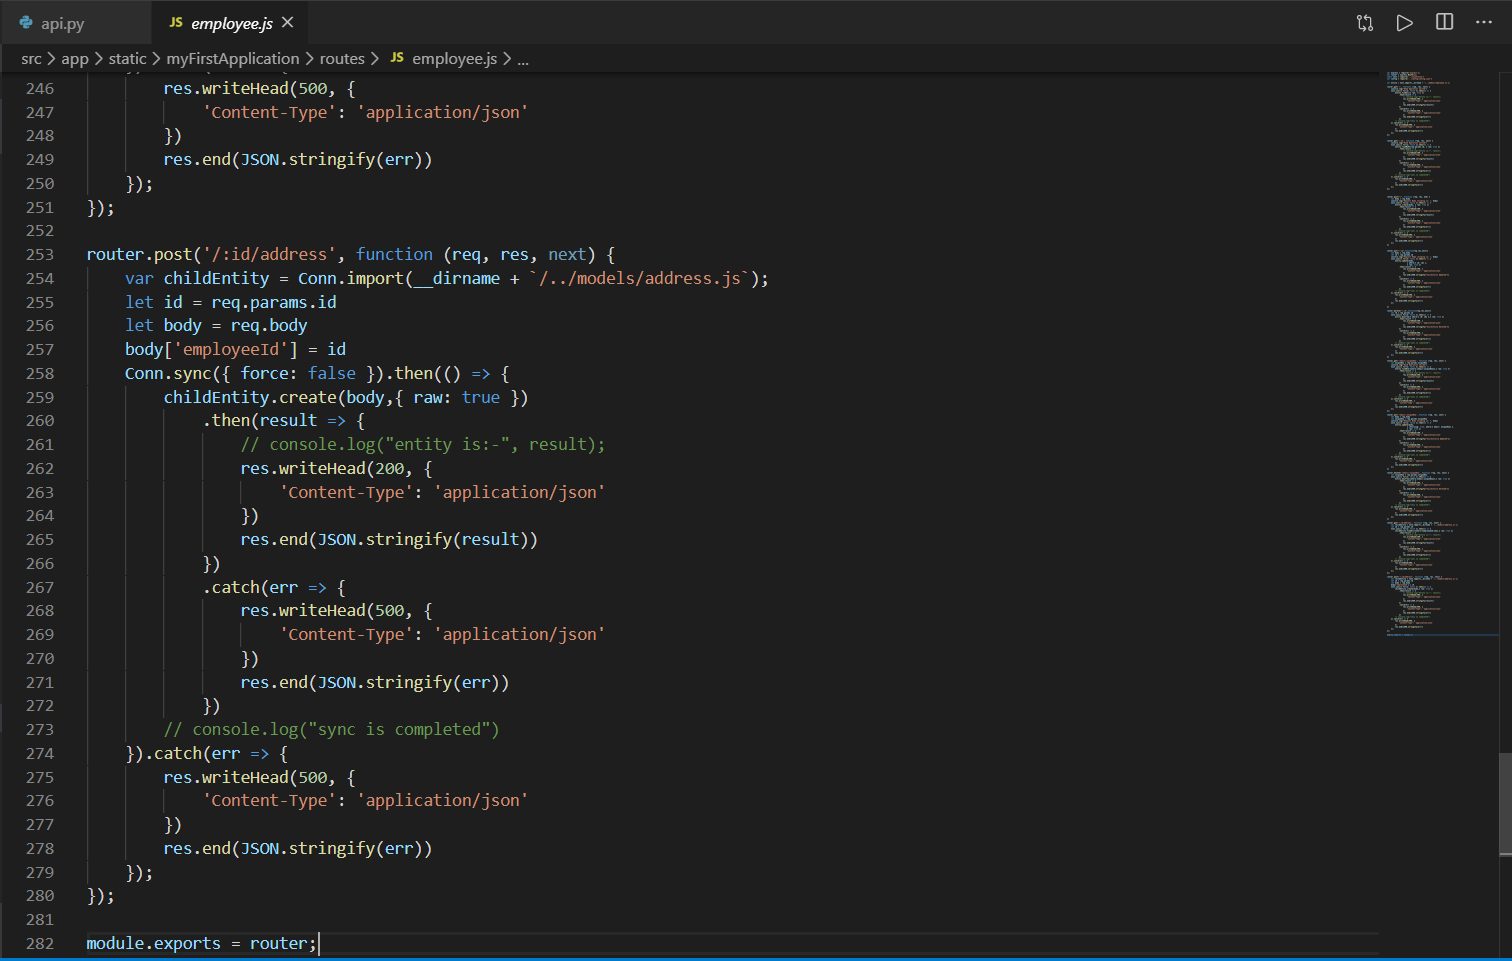
\includegraphics[scale=0.215]{./fig9.png}
   \caption{Generated code from the skeleton}
   \label{fig:my_label}
\end{figure}

Once the whole operation from generating models to generating code is completed, the application creates a zip file of the generated code readily available for the user to download.

\section{DEPLOYMENT AND MAINTENANCE}
\subsection{Deployment}
The architecture diagram briefly explains the components in our project. We can divide the architecture in different planes viz. the management plane, API plane and the storage plane. We have to do the deployment and maintenance of our interaction server. Which is the management plane in our architecture. User would interact with this as it would be hosting the front end and rest of the deployments are to be done at the users end.
\subsubsection{Management Plane}
For the management plane, we have the management server hosted in cloud on a docker hub having resilient kubernetes cluster serving the APIs. The management plane is further divided in 2 servers the front end server and the API server i.e. the docker hub. The front end server hosts our React application and the API server provides us the APIs
\subsubsection{Storage Plane}
The deployment of the interaction plane would be done after the deployment of storage plane. The storage plane will basically have the database servers which user wants for their application. The user needs to have the sql client server installed on the server and can use any deployment strategy and storage strategy for their database. The user just needs to provide the important credentials of the database to create tables in the database and do all the important changes required in their database and get APIs for content of database.
\subsubsection{Interaction Plane}
The interaction plane is the plane in which the user will host the APIs generated by us. Once the user has connected his database with the management plane and launched the application the completed code for the APIs would be ready also the Dockerfile required for the same would be ready. the user just has to download the zip and launch the node application or create an image of the Dockerfile and spawn a container of that dockerfile.
To deploy the interaction plane user can decide his own strategy and device his own architecture. User can have single server hosting the APIs in the node app or user can also have kubernetes cluster inside a docker hub or a basic docker container running the APIs this would be the interaction plane with single server or multiple server deployed by the user.


\begin{figure}[h]
   \centering
   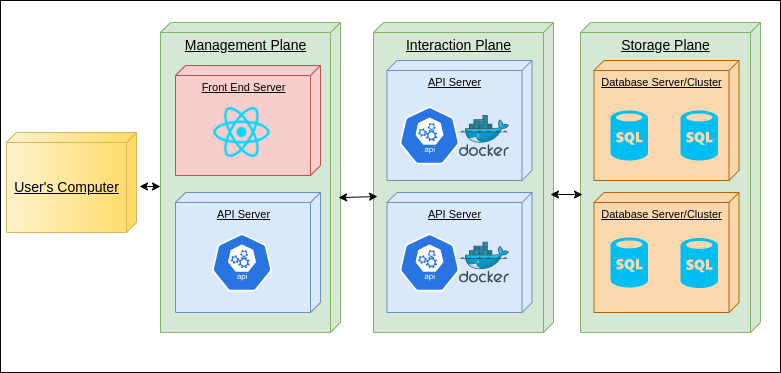
\includegraphics[scale=0.27]{./DeploymentDiagram.png}
   \caption{Deployment Diagram}
   \label{fig:my_label}
\end{figure}

\subsection{Maintenance}
The responsibility of deployment of management plane is with us and so will be the responsibility of maintaining the management plane is ours. For the maintenance of management we need to keep the servers always reachable up and running so that we always have a user input. To maintain the management plane with every bug fix or new change we will have to  update the code on the front end server if we have changes in front end. For the other changes in APIs we will have to build a docker image with the latest code and change the pods in the kubernetes cluster to use the updated docker image.

The other planes are deployed by the user so the maintenance is also users responsibility. For the storage plane once the user has deployed it with a required architecture user can make all the changes in the schema of database using the management UI as we can connect to the Database and make any changes required in the database.For maintenance of the interaction plane if the user wants to change the database or re deploy the APIs or make any changes in API code he just needs to make the required change himself. So the steps to keep the interaction plane updated is the user need to make the changes in database using the UI and download the latest code once the code is downloaded and updated by making any changes in code the user must again the deploy code in the server and start the API server or generate the docker image of the latest updated code and use the docker image to spawn containers or in the kubernetes cluster according the user requirements.

\section{EVALUATION}
\subsection{Evaluation Methodology}
The main goals of our application are building the application, building databases and generating the code.
We have evaluated our application on these parameters by using different methods. We followed the following methods:
\begin{enumerate}
  \item We gave our application to different professionals like back-end developers, data scientists, and different non technical people and collect the evidence for evaluation. The users evaluated our application on the performance quality. They filled a grid of specifications for the performance. Table 1 represents the mean of all the users values. We gave the following metrics:
  \begin{itemize}
    \item Usability: The user used our application for their particular use case. We gave the steps to some users and take their evaluation. The user connected/built the database, generate code and host the application. 
    \item Speediness: The users evaluated this metric by how fast they were able to achieve their use case. Evaluating this part was a little tricky. If the user started building the database and then built the application, then the speed was a little slow. But if the users connected to an existing database and then built the application, then it was created in just a few seconds.
    \item Efficiency: The users evaluated this metric by how efficient our application is. The user checked how efficient our generated code is. How many lines are present. How good the code structure is. Are all the CRUD operations that the user want in our code. How bug free our code is and how RESTful it is.
  \end{itemize}
  \item We compared our application with the existing code generators. We compared them with xmysql[15], sandman[16] and util-raml-code-generator[22]. We had a predefined metrics for this evaluation also. We evaluated all the applications on the following features:
  \begin{itemize}
    \item Code Quality: Once the code is generated, we evaluated how bug free the code is, how good the file structure is, how many lines of code are present, and how accessible, editable and modifiable the code is. 
    \item Database Connectivity: We evaluated how easy it is to integrate the users existing database or create new databases, edit tables and create complex relationships.
    \item Cloud Services: We evaluated how easy it is to host the code provided these applications.
  \end{itemize}
\end{enumerate} 
\subsection{Performance and Benchmarks}
\begin{itemize}
    \item Usability: 10 users tried to create rest API's using all the 4 applications. 9 users were able to successfully create the API's using EBaaS. Fig 14 shows the comparison of all the 4 applications. Util-raml was a little complicated as the user had to create the raml file. 4 out of 10 users were able to generate API's using that. Sandman2 and xmysql performed quite similarly. Users with prior technical background were easily able to launch the API's but users with non technical background faced challenges. 7 out of 10 users were able to launch API's using Sandman and  8 out of 10 users were able to launch using xmysql.
    \begin{figure}[h]
   \centering
   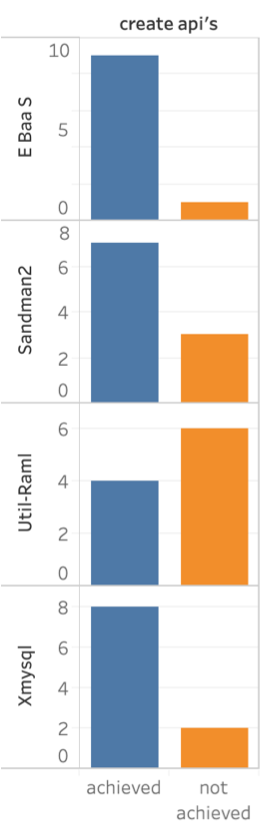
\includegraphics[scale=0.33]{./CreateApis.png}
   \caption{Usability to Create API's}
   \label{fig:my_label}
\end{figure}
    \begin{table}[]
\begin{tabular}{|l|c|c|c|c|}
\hline
                      & \multicolumn{1}{l|}{util-raml} & \multicolumn{1}{l|}{xmysql} & \multicolumn{1}{l|}{sandman2} & \multicolumn{1}{l|}{EBaaS} \\ \hline
Usability             & 2/5                            & 3/5                         & 3/5                           & 5/5                        \\ \hline
Speediness            & 2/5                            & 5/5                         & 5/5                           & 4/5                        \\ \hline
Efficiency            & 3/5                            & 2/5                         & 2/5                           & 4/5                        \\ \hline
Code Quality          & 4/5                            & N/A                         & N/A                           & 4/5                        \\ \hline
Database Connectivity & N/A                            & N/A                         & 4/5                           & 4/5                        \\ \hline
Cloud Services        & N/A                            & 4/5                         & 4/5                           & 5/5                        \\ \hline
\end{tabular}
\caption*
\end{table}
    \item Speediness: We tracked the average times to launch the API's for different use cases. The use case to connect to an existing database was common for all the applications. Util-raml performed quite slow as the users had to create a raml file for their database and give that file to the code generator. It took around 4.3 mins to create API's using util-raml. Xmysql, sandman2, and EBaaS performed had nearly the same speed. It took around 12 seconds to launch the applications. Fig 15 shows the comparison between different applications.
    
    
\begin{figure}[h]
   \centering
   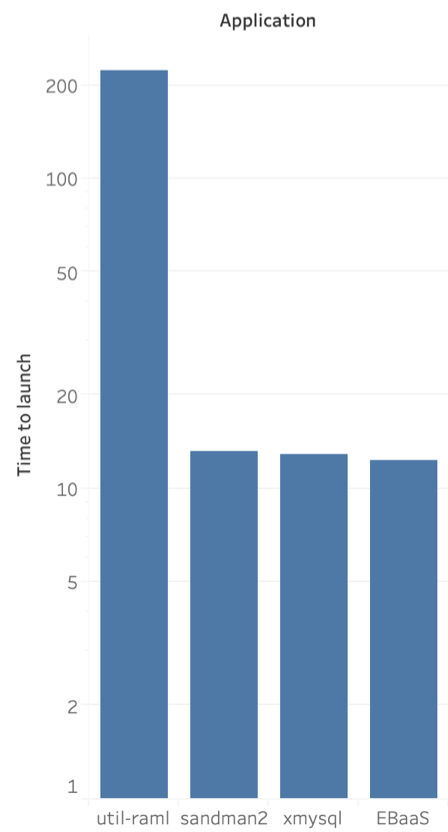
\includegraphics[scale=0.33]{./TimeToLaunch.png}
   \caption{Time to launch an Application}
   \label{fig:my_label}
\end{figure}

    \item Code Quality: xmysql and Sandman2 does not give code. So we did not add them in this comparison. Util-raml and EBaaS both performed pretty good. For the same use case, util-raml had 102 lines of code for entities and 166 lines of code for services. While EBaaS had 26 lines of code for entities and 143 lines of code for services. Both the code generated were quite modifiable. Util-raml gave the code in PHP and JavaScript while EBaas generated the code in JavaScript. Fig. 16 shows the comparison between the different applications on the basis of lines of code.
    
\begin{figure}[h]
   \centering
   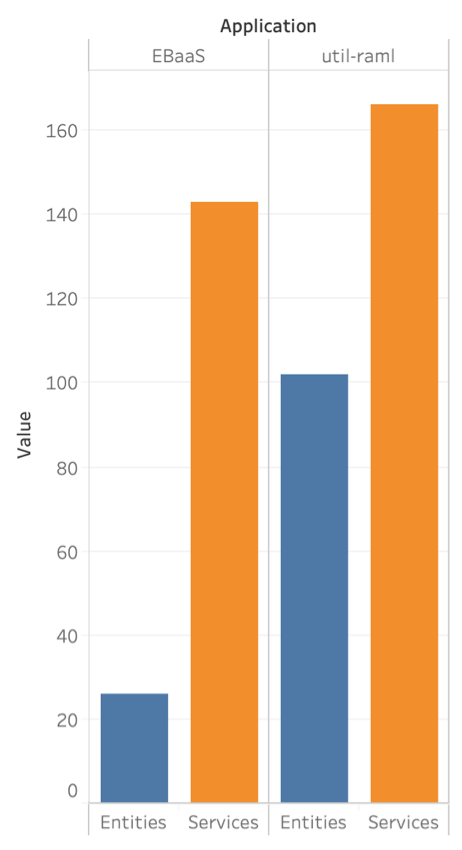
\includegraphics[scale=0.33]{./LinesOfCode.png}
   \caption{Lines of Code}
   \label{fig:my_label}
\end{figure}

\begin{figure}[h]
   \centering
   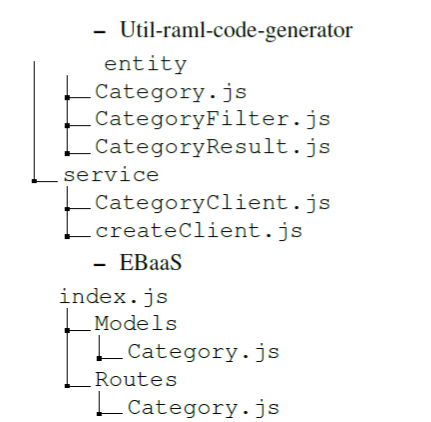
\includegraphics[scale=0.50]{./Structure.PNG}
   \caption{File Structure Comparison}
   \label{fig:my_label}
\end{figure}
    
    \item Database Connectivity: EBaaS performed the best here. EBaaS supported database connectivity from existing databases, and also gave access to create new databases from scratch or by uploading a sql file or excel file. It was difficult to connect to database in util-raml because the user had to create the raml files. xmysql and Sandman2 takes the database string in the parameters. They do not give features to create a new database or modify an existing database. Sandman2 supports many different types of databases. EBaaS only supports MySQL databases.
    \item Cloud Services: The world is quickly moving towards cloud computing which allows software to be available based on demand. To make it even more feasible, containerization has taken its own place allowing to provide better security, portability, fast deployment amongst other benefits. Keeping this in mind, EBaaS provides a docker file on hand which provides users to easily make their backend application containerized. Even though, Xmysql and Sandman2 provides docker support, Util-raml-code-generator fails to do so.
 \end{itemize}

      





\section{CONCLUSION}
EBaaS is basically a one stop application for developing and maintaining the complete back end of any application. Interacting with the UI, user can develop and database, make updates in the database and have the API code ready to integrate the APIs with their own front end. User with their own servers can have the complete, efficient and speedy back end with all basic APIs ready with just few clicks and inputs. User can later make any changes in the API code provided by our code generator to also have user defined APIs. So EBaaS basically as the name suggested is an application to provide enterprise backed as a service.
\section{FUTURE WORK}
This project currently focuses on the connection/Creation of the relational databases based on which it is generating the RESTful APIs.In future the scope of the project can be expanded to the Non Relational databases. This project has so much scope of incorporating ML Services which can be used later on for recommendation based on the use case. For example, if the use case involves sales then a ready to use ML API service to gain insights into the sales and much more.
Currently, this project is reserving REST web architecture for generating the back-end code, it could be made even more useful by giving users the option of selecting different architectures like GraphQL, SOAP, RPC etc. When it comes to automation, the work, research and innovation is never going to stop and hence the future capabilities of this project can also be infinite. 

\begin{thebibliography}{99}

\bibitem{c1} (November 30, 2018 Friday).Technavio Updates on the Global Backend as a Service Market. Professional Services Close-Up. Retrieved from \href{https://advance.lexis.com/api/document?collection=news&id=urn:contentItem:5TVM-M141-F06S-P1FM-00000-00&context=1516831}{Link}
\bibitem{c2} Costa, Igor, Jean Araujo, Jamilson Dantas, Eliomar Campos, Francisco Airton Silva, and Paulo Maciel. 
``Availability Evaluation and Sensitivity Analysis of a Mobile Backend‐as‐a‐service Platform.'' Quality and Reliability Engineering International 32.7 (2016): 2191-205.
\bibitem{c3} T. Haselmann, G. Thies and G. Vossen, ``Looking into a REST-Based Universal API for Database-as-a-Service Systems'', 2010 IEEE 12th Conference on Commerce and Enterprise Computing, Shanghai, 2010. URL: \href{http://ieeexplore.ieee.org/stamp/stamp.jsp?tp=&arnumber=5708388&isnumber=5708385}{Link}
\bibitem{c4} J. Nazdrowicz, "A relational database environment for numerical simulation backend storage," 2015 22nd International Conference Mixed Design of Integrated Circuits \& Systems (MIXDES), Torun, 2015. URL: \href{http://ieeexplore.ieee.org/stamp/stamp.jsp?tp=&arnumber=7208595&isnumber=7208464}{Link}
\bibitem{c5} Kolovos, D. et al.: Epsilon (Jul 2015), http://www.eclipse.org/epsilon
\bibitem{c6} S. Ceri, P. Fraternali, and A. Bongio. Web Modeling Language (WebML): a Modeling Language for Designing Web Sites. J. Comp. Netw., 33:137–157, 2000.
\bibitem{c7} Prajak Chertchom, Shigeaki Tanimoto, Hayato Ohba, Tsutomu Kohnosu, Toru Kobayashi, Hiroyuki Sato, Atsushi Kanai, Software Engineering, Artificial Intelligence, Networking and Parallel/Distributed Computing, vol. 721, pp. 107, 2018.
\bibitem{c8} R. T. Fielding. Architectural Styles and the Design of Network-based Software Architectures. PhD thesis, 2000.
\bibitem{c9} N. Koch and S. Kozuruba. Requirements models as first class entities in model-driven web engineering. In ICWE Workshops, pages 158–169, 2012.
\bibitem{c10} Blog.v soft consulting.com. (2019). Swagger (OAS) vs. RAML - Which is Better for Building APIs?
\bibitem{c11} X. Qafmolla and V. C. Nguyen. Automation of Web Services Development Using Model Driven Techniques. In ICCAE conf, volume 3, pages 190–194, 2010.
\bibitem{c12} Zenqry.com. (2019). ZenQuery - Enterprise Backend as a Service.
\bibitem{c13} GitHub Paysera. (2019). paysera/util-raml-code-generator.
\bibitem{c14} https://blog.risingstack.com/node-hero-node-js-project-structure-tutorial/
\bibitem{c15} https://github.com/o1lab/xmysql
\bibitem{c16} https://github.com/jeffknupp/sandman2
\bibitem{c17} A. Schauerhuber, M. Wimmer, and E. Kapsammer. Bridging Existing Web Modeling Languages to Model-driven Engineering: A Metamodel for WebML. In ICWE conf., 2006.
\bibitem{c18} WebRatio. https://www.webratio.com/site/content/en/web-application-development (last accessed on April. 2020)
\bibitem{c19} Hamza Ed-douibi, Javier Luis Cánovas Izquierdo, Abel Gómez, Massimo Tisi, and Jordi Cabot. 2016. EMF-REST: generation of RESTful APIs from models. In Proceedings of the 31st Annual ACM Symposium on Applied Computing (SAC ’16). Association for Computing Machinery, New York, NY, USA, 1446–1453.
\bibitem{c20} Liu, Y., Wang, Q., Zhuang, M., Zhu, Y.: Reengineering Legacy Systems with RESTful Web Service. In: 2008 32nd Annual IEEE International Computer Software and Applications Conference (2100219007), pp. 785–790 (2008)
\bibitem{c21} Crocombe, R., & Kolovos, D. S. (2015, September). Code Generation as a Service. In CloudMDE@ MoDELS (pp. 25-30).
\bibitem{c22} https://github.com/paysera/util-raml-code-generator
\end{thebibliography}
 



\end{document}
